\documentclass[./thesis.tex]{subfiles}

 
\begin{document}
\label{chap:CIPSI}

Need to have a list of reasonable size = need a general way to select determinants. 

Unlike for Davidson, connections aren't inside a given set but by an intermediary external determinant $\alpha$ or $\ket \alpha$ ...; 

=======

'alpha' = like creating PSI, apply excitation masks on generators. in CIPSI, "full\_generators". \\
approximate by taking only biggest generators/selectors. Very qualitative, no big deal \\
first idea : disconnect "a priori" a piece of wavefunction ( minilist ). ?\\
Balance between size of sample VS size of removed piece of wavefunction. \\
by extension, iterative filtering ( generator, first hole, second hole ) \\
then, have some systematic definition of alpha / I ( microlist ). \\
avoid explicitely comparing I and alpha ( feuille de PQ ). \\

==========



\begin{algorithm}
	\caption{Simple CIPSI}
		\KwData{ $\Psi$ }
		\KwResult{ Guarantees all $\epsilon(\alpha)$ are computed a single time. }
		\For {$g \gets 1, N_{det}$}{
		\ForAll {$\ket \alpha$ ; $\langle D_g | H | \alpha \rangle \neq 0$}{
		\tcc{apply all double excitations on $|D_g \rangle$}
		\For{$p \gets 1, g-1$}{
			\If{$\ket \alpha$ connected to $D_p$}{
				\tcc{$\ket \alpha$ has already been generated by $D_p$}
				Break loop over $\ket \alpha$ \;
			}
		}
		 $R \gets 0$ \;
		\For{$s \gets g, N_{det}$}{
			\If{$D_s==\alpha$}{
				Break loop over $\ket \alpha$
				%\Comment $\alpha \in \Psi$
			}
			 $R \gets R + \Hij{D_s}{\alpha}$ \;
		}
		 assert $R == \Hij{\Psi}{\alpha}$  \;
		 $\epsilon(\alpha) = \frac{R^2}{\Delta E_\alpha}$
		}
		}
\end{algorithm}

\section{def}

\section{notation(?)}


\begin{equation}
\Psi = \sum_I {c_I | D_I \rangle}
\end{equation}


Indices $p,q,r,s$ refer to SPINorbitals, $p$ and $r$ being of same spin, $q$ and $s$ being of same spin. 


$G = D_I$ generator determinant

$S = D_J$ selector determinant

$\alpha$ external determinant

\section{base issue}
As can be told by the formula of $\epsilon(\alpha)$, selection requires to enumerate all connections between all internal and all external determinants.
The simplest solution to achieve this, would be using an ``internal to external'' approach.
\begin{itemize}
\item
loop over generators $\ket G$
\item
loop over double excitations $\hat T$
\item increment $\epsilon(\alpha = \hat T \ket G \notin \Psi)$ accordingly.

\end{itemize}
Unfortnately, keeping track of all $\epsilon(\alpha)$ at the same time is not feasible, since their numbers scales as $\Ngen \times \mathcal{O}_{virt}^2 \times \mathcal{O}_{occ}^2$.


\section{Previous version}

Originally, the quantum\_package had straighforward ``external to internal'' approach, solving the problem of keeping track of all $\epsilon(\alpha)$ at the same time. The external space was created as indicated in \alert{creating subspace}, by checking connection to a previous generator. Because the space we consider is either Full CI or CAS-SD, we do not need to check whether the connection is authorized by bitmasks  \alert{A EXPLIQUE DANS create subpace}, since this will always be the case. Then, $\Hij{\alpha}{\Psi}$ was computed individually for each $\kalpha$ by comparing it to all selector determinants.

\begin{itemize}
\item
loop over generators $\ket G$
\item
generate all determinants connected to $G$
\item
from this set, discard those that appear in $\Psi$. This is now a set of $\ket \alpha$
\item
from this set, discard those that have already been generated before, i.e. those connected to $D_K$ with $K<I$. This is now a set of unique $\ket \alpha$.
\item
compute $\epsilon(\alpha) = \frac{\langle \alpha|H|\Psi\rangle^2}{\Delta E_\alpha}$ for those new $\ket \alpha$
\end{itemize}

\begin{figure}[h!]
	\begin{center}
		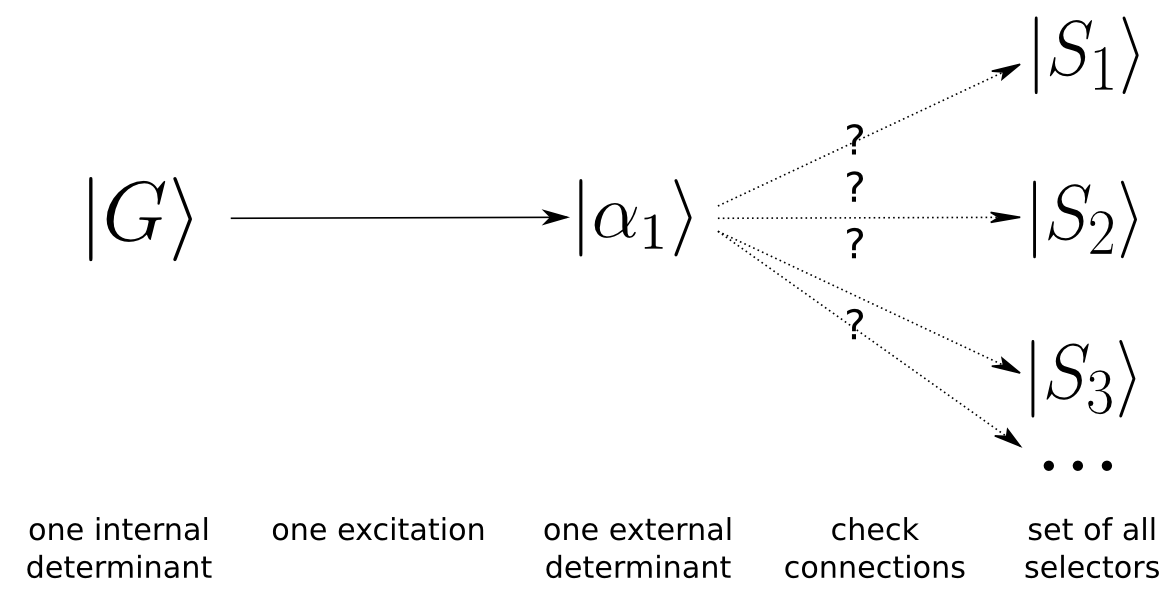
\includegraphics[width=0.7\columnwidth]{figures/cipsi/old_cipsi}
		\caption{{\label{selexemple2}%
		}}
	\end{center}
\end{figure}


\section{Current version base idea}

The current approach is intermediate between computing $\epsilon(\alpha)$ one by one, and keeping track of all of them at the same time.
It creates a subset, or ``batch'' of determinants small enough to fit into memory, and importantly, that is implicitely defined rather than arbitrary.
A batch is defined by a doubly ionized generator


\begin{equation}
G_{pq} = a_p a_q G
\end{equation}



Determinants contained in the $G_{pq}$ batch , some of which may be unique $\ket \alpha$, can be systematically defined by two indexes $r$ and $s$ with

\begin{equation}
a^\dagger_r a^\dagger_s a_p a_q  G = G^{rs}_{pq}
\end{equation}

Essentially, determinants in a batch are defined by their difference to $G_{pq}$. Therefore, comparing $G_{pq}$ to a selector determinant, allows to systematically determine which $\kalpha$ of the batch it will connect to, and by what excitation. Additional filtering mechanism are set up, that will be explicited later on.

\begin{figure}[h!]
	\begin{center}
		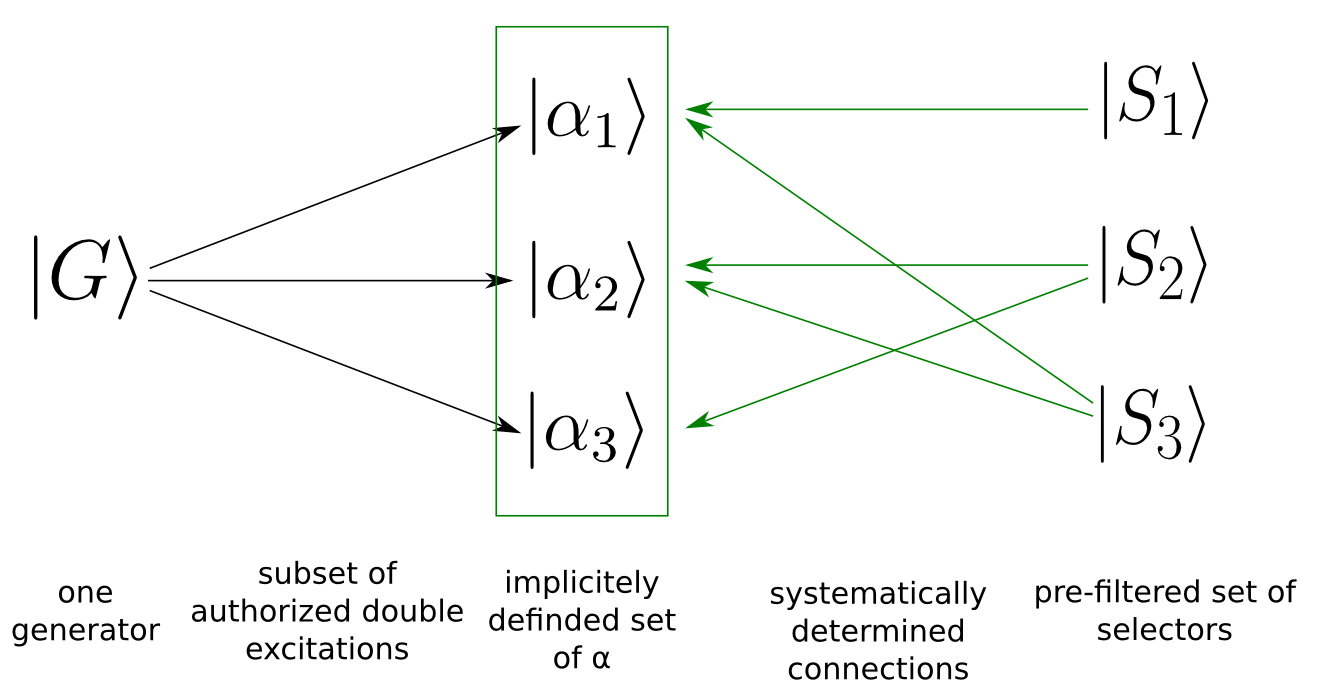
\includegraphics[width=0.7\columnwidth]{figures/cipsi/new_cipsi}
		\caption{{\label{selexemple2}%
		}}
	\end{center}
\end{figure}

\subsection{Unoptimized algorithm}

A simplified version of the algorithm goes as follow. It makes no approximation and ignores the filtering and loop breaking optimizations.



\begin{algorithm}
	\caption{UNBLOCK\_SINGLE}
	\label{alg:unblock_single}
		\KwData{ -------}
		\KwResult{ -------------}
		

		\If{($q$ is of spin $\alpha$) and ($p=M_\beta$)}{
				$B_{*,M_\beta} \gets TRUE$ \;	
				$B_{M_\beta,*} \gets TRUE$ \;		
			}
			
			\If{($p$ is of spin $\beta$) and ($q=M_\alpha$)}{
				$B_{*,M_\alpha} \gets TRUE$ \;	
				$B_{M_\alpha,*} \gets TRUE$ \;		
			}
\end{algorithm}


\begin{algorithm}
	\caption{simplified CIPSI}
	\label{alg:selection}
	\KwData{ $\Psi$}
	\KwResult{ $\Hij{\alpha}{\Psi} \neq 0$ has been computed exactly once for any $\alpha \notin \Psi$ }
		
	\For{$g \gets 1, t_g$}{
	$M_\alpha \gets$ any $\alpha$ spinorbital occupied in $D_g$ \;
	$M_\beta \gets$ any $\beta$ spinorbital occupied in $D_g$ \;
	\ForAll{$(p,q) ; a_p a_q D_g \neq 0$}{
		$G_{pq} \gets a_p a_q D_g$\;
		$B$ a logical matrix size $N_{sorb} \times N_{sorb}$ \;
		$P$ a real matrix size $N_{sorb} \times N_{sorb}$ \;
		\tcc{$B$ and $P$ are indexed by spinrobitals}
		$B_{*,*} \gets TRUE$ \;
		$P_{*,*} \gets 0$ \;
		\ForAll{$r ; (a_r G_{pq} = 0)$ or $(r=p)$ or $(r=q)$}{
          		$B_{*r} \gets FALSE$ \;
          		$B_{r*} \gets FALSE$ \;
		}
		
		\tcc{unblocks some elements of $B$ so that single excitations are properly generated}
		Unblock\_single($B$, p, $q$, $M_\alpha, M_\beta$)
			
				
			
		\For{$p \gets 1,N_{det}$}{
			$S \gets D_p$ \; 
			$c \gets iand(S, not(G_{pq}))$ \; 
			\If{$popcnt(c) = 2$}{
				$e \gets LIST\_FROM\_BITSTRING(c)$\; 
				$B_{e_1, e_2} \gets FALSE$\; 			  
			}			
			\tcc{see table XXX for the loops}
			\uIf{$p < g$}{
				    
				\ForAll{$(\tilde r, \tilde s) ; \Hij{S}{G_{pq}^{\tilde r \tilde s} \neq 0}$}{
				  $B_{rs} \gets FALSE$ \;
				} 
			}
			\uElseIf{$p \leq t_s$}{
				\ForAll{$(\tilde r, \tilde s) ; \Hij{S}{G_{pq}^{\tilde r \tilde s} \neq 0} ; B_{rs}$ }{
				  $P_{rs} \gets P_{rs} + \Hij{a^\dagger_r a^\dagger_s G_{pq}}{S}$ \;
				}
			}
		}
		\ForAll{$(r,s);B_{rs}$}{
		  assert $P_{rs} = \Hij{a_r^\dagger a_s^\dagger G_{pq}}{\Psi}$ \;
		}
	}
	} 
\end{algorithm}

\begin{itemize}
\item
\textbf{generator loop} : outer loop over $D_I$
\item
$G = D_I$
\item
Iterate over all possible $G_{pq}$

\item
allocate an empty matrix $P(G_{pq})$ indexed by $r$ and $s$. Each cell is associated with $G^{rs}_{pq}$. Some cells will be tagged (in whatever way) as not containing a unique $\ket \alpha$ ; they can contain either
\begin{itemize}
\item
a determinant present in the wavefunction
\item
a non-existing determinant
\item
a non-unique $\ket \alpha$ ( either a bi-excitation of a previous generator, or a single excitation of the current one )
\end{itemize}

\item
Since two electrons cannot occupy the same spinorbital, tag cells where $r$ or $s$ is occupied in $G_{pq}$ ( tags non-existing determinants ). 
\item
apply single excitation tagging : this is described - what a surprise - in section "single excitation tagging". ( tags duplicate $\ket \alpha$ ). This ensures single excitations for $G$ are generated exactly once.
\item
\textbf{selector loop} : inner loop over $D_J$ 
\item
$S = D_J$
\item
Systematically determine whether there is an $r,s$ pair so that $S=G_{pq}^{rs}$. In other words, look for $S$ in the current batch. If there is, tag the corresponding cell. ( tags determinants present in the wavefunction )
\item
Systematically determine $r,s$ pairs so that $G_{pq}^{rs}$ is connected to $S$
\item
If $J<I$, tag the corresponding cells ; $G_{pq}^{rs}$ has already been generated by $S$ ( tags duplicate $\ket \alpha$ )
\item
If $J \geq I$, increment all untagged $P_{r,s}(G_{pq})$ matrix element by $\Delta P_{r,s}(G_{pq}) = c_J\langle S| H|  G^{rs}_{pq} \rangle$. Note that $\overrightarrow{T}$ so that $S=\overrightarrow{T}G^{rs}_{pq}$ can be systematically deduced at the same time as the $r,s$ pair.
\item
End of loops. All untagged cells are guaranteed to contain a unique $\ket \alpha$, and $P_{r,s}(G_{pq}) = \langle \Psi |H|G^{rs}_{pq} \rangle$, thus\\

\begin{equation}
\epsilon(G_{pq}^{rs}) = \frac{P_{r,s}(G_{pq})^2}{\Delta E_{G^{rs}_{pq}}}
\end{equation}

\end{itemize}


\subsection{Tagging}

Tagged cells are simply tracked using a logical matrix $B(G_{pq})$.
In some cases, full columns/rows are to be tagged. For performance purpose, it's useful to allocate a boolean vector to track fully tagged columns, and another to track fully tagged rows. While important, this optimization is fairly simple to set up and use, so for simplification purpose, it will be mostly ignored.


\subsection{Single excitation tagging}

The algorithm is designed to generate all $G_{pq}^{rs}$, which are doubly excited from $G$. The singly excited determinants are not explicitly generated, but are formally present as $G_{pq}^{ps}$.
An issue is that $G_{pq}^{ps}$ refers to the same determinant $G_q^s$ regardless of $p$, and the algorithm only tags a $\ket \alpha$ as duplicate if it has a previous generator $K$, i.e. if

\begin{equation}
G_{pq}^{rs} = {K}_{p'q'}^{r's'} ; K = D_{I'<I}
\end{equation}

It doesn't cover the case $G_{pq}^{ps} = G_{p'q}^{p's}$.
We default to tag $G_{pq}^{ps}$, which prevents generating single excitations, and selectively untag in certain cases:


\begin{itemize}
\item
Untagging all $\alpha$ single excitations of $G$ exactly once:

Pick $P$ any non-frozen $\beta$ spinorbital occupied in $G$. Untag $G_{Pq}^{Ps}$ whenever $q,s$ are of spin $\alpha$. Any $\alpha$ single excitation $q \rightarrow  s$ is untagged a single time.

$P$ cannot be of spin $\alpha$, because single excitations $P \rightarrow  s$ and $q \rightarrow  P$ would be formally present as $G_{PP}^{Ps}$ and $G_{Pq}^{PP}$, which aren't ever generated, since for obvious reasons the algorithm never considers $G_{qq}$ or $G_{pq}^{rr}$.
\item
Untagging all $\beta$ single excitations exactly once:

Pick $Q$ any $\alpha$ spinorbital occupied in $G$. If $p,q$ are of spin $\beta$, untag $G_{pQ}^{rQ}$. Any $\beta$ single excitation $p \rightarrow  r$ is untagged a single time.
\end{itemize}


\section{Approximation}

This method performs an exact CIPSI. However, given the qualitative nature of this procedure, it is possible to save a vast amount of calculation with minimal approximation.

Determinants $D_I$ being sorted by decreasing absolute values of $C_I$. Two assumptions are made :
\begin{itemize}
\item
It is very unlikely $\ket \alpha$ will be selected if it's not connected to any $D$ with a large coefficient. This approximation is achieved by setting threshold $t_g$ and limiting the generator loop to $D_{I \leq t_g}$.
\item
Connections to $D$ of small coefficient can be neglected. We do not need accurate values for $\epsilon(\alpha)$, small differences are unlikely to substantially change the subset of the largest ones. This approximation is achieved in a similar way by limiting the selector loop to $D_{J \leq t_s}$ with $t_s \geq t_g$.
\end{itemize}

Note that generator determinants are a subset of selector determinants.
A new loop must be created over $D_{J > t_s}$, since any $G_{pq}^{rs}=D_{J > t_s}$ must still be tagged for being present in the wavefunction.

\begin{figure}[h!]
	\begin{center}
		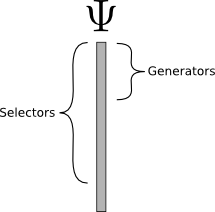
\includegraphics[width=0.4\columnwidth]{figures/cipsi/selexemple2}
		\caption{{\label{selexemple2}%
		}}
	\end{center}
\end{figure}






\section{Systematic determination}

The systematic determination of connections between $S$ and determinants from the $G_{pq}$ batch is done by comparing $S$ to the double ionized determinant $G_{pq}$. This yields a set of differences. Remembering $S$ has two extra electrons compared to $G_{pq}$, there are 4 cases of interest:
\begin{itemize}

\item
$i$,$j$ are occupied in $S$ but not in $G_{pq}$
\item
$i$,$j$,$k$ are occupied in $S$ but not in $G_{pq}$ ; $a$ is occupied in $G_{pq}$, but not in $S$
\item
$i$,$j$,$k$,$l$ are occupied in $S$ but not in $G_{pq}$ ; $a$,$b$ are occupied in $G_{pq}$, but not in $S$
\item
More differences : $S$ isn't connected to any $G_{pq}^{rs}$ and can be ignored. 

\end{itemize}

Based on these indices, it's possible to immediately deduce any $r,s$ pair so that $G_{pq}^{rs}$ is at most a double excitation of $S$, as well as the excitation operator $\overrightarrow{T}$ so that $G_{pq}^{rs}=\overrightarrow{T}S$. figure XXX shows two possible cases as example.

Taking spin into account, there are 10 possible cases, listed in table ???.


It's noticeable that, because of the "wildcard" indices $X$ and $Y$ :
\begin{itemize}

\item
Cases of the form $a,ijk$ cause full rows/columns of $P(G_{pq})$ to be tagged or incremented.
\item
Cases of the form $ij$ cause the whole $P(G_{pq})$ matrix to be tagged or incremented. Obviously, tagging the whole matrix means stopping the computation for $G_{pq}$.
\end{itemize}

\begin{figure}[h!]
	\begin{center}
		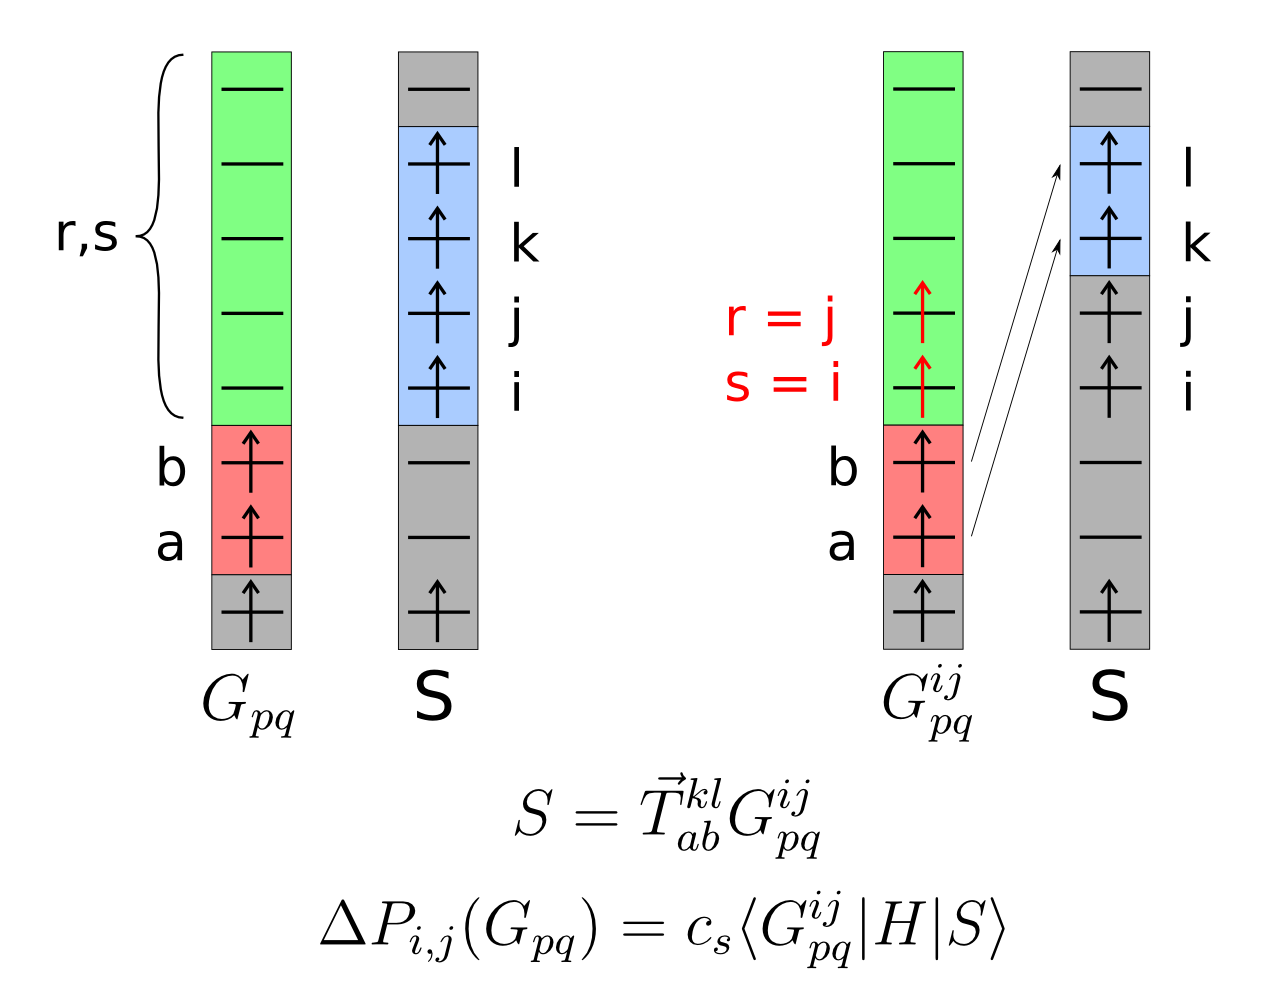
\includegraphics[width=0.70\columnwidth]{figures/cipsi/systematic_determination}
		\caption{{Replace this text with your caption%
		}}
	\end{center}
\end{figure}
\begin{figure}[h!]
	\begin{center}
		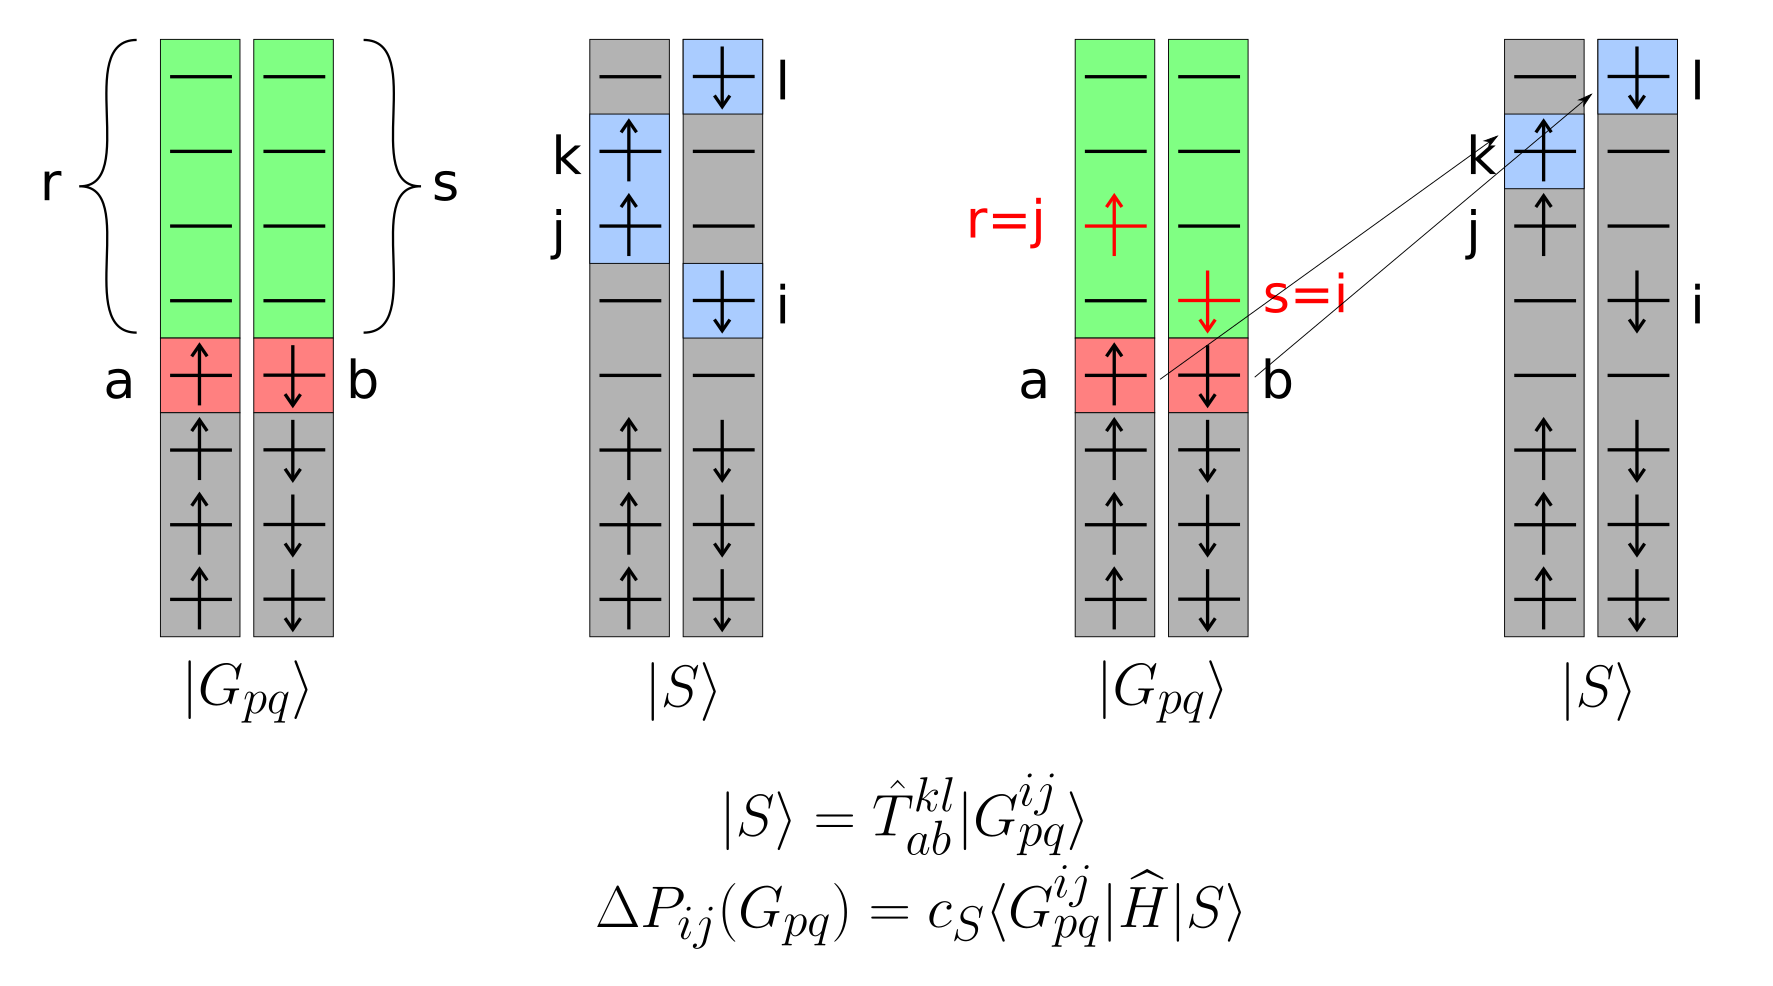
\includegraphics[width=0.70\columnwidth]{figures/cipsi/systematic_determination2}
		\caption{{\label{splash}%
		}}
	\end{center}
\end{figure}

\section{Filtering and loop breaking}
A great deal of processing power is lost, because every doubly ionized generator $G_{pq}$ is compared to all selector determinants. In the vast majority of cases, it will show no connection can be made and the selector will be ignored. Thus, it's interesting to filter selector determinants in more outer loops ( generator loop, and loop over first ionization ).

This can be done using the distance $f_A^B = f_B^A$, defined as the minimal number of operations - moving, annihilating or creating an electron - that must be done to go from a determinant $A$ to a determinant $B$ with ionization degrees of respectively $a$ and $b$. B



\begin{equation}
f_A^B = \frac{||A_\alpha \oplus B_\alpha|| + ||A_\beta \oplus B_\beta|| + |a-b|}{2}
\end{equation}


Considering $S$ a selector determinant and $X$ a generator determinant in a state of ionization from 0 to 2 ( it essentially is a wildcard for $G$, $G_p$ or $G_{pq}$ ).

\begin{itemize}
\item
$f_X^\alpha + f_\alpha^S \geq f_X^S$
\item
$\ket \alpha$ can be generated from $X$ if and only if $f_X^\alpha \leq 2$
\item
$\ket \alpha$ is connected to $S$ if and only if $f_\alpha^S \leq 2$
\item
$0 \leq (f_{a_p X}^S - f_X^S) \leq 1$
\end{itemize}

(detailler?)
From the rules above, we can deduce that given any $X$ and $S$, there exists a $\ket \alpha$ generated from $X$ so that $\Hij{\alpha}{S} \neq 0$ only if $f_X^S \leq 4$.

Based on this, a filtering system can be set up, as shown on figure \ref{fig:selection}.\\

The diagram is a bit complex and deserves comments. 
It shows a triple loop : over generators ($G$) ; then over $p$ a first ionization ($G_p = a_p G$) ; then over $q$ a second ionization ( $G_{pq} = a_p a_q G$ ). The variational determinants "flow" from the top $\Psi$ into intermediate lists, that are fully constructed before proceeding to the inner loop, as they will be the "sources" of determinants for that inner loop.
A selector can only be duplicated at the node denoted by a black circle. Otherwise, it follows a single path, always going for the horizontal path if it satisfies the associated condition.
If it doesn't satisfy the condition of an horizontal path, and there is no further vertical path, it is discarded.

This diagram features $DROP$ instructions. Those are reached when, predictably, the current loop iteration will not yield any unique $\ket \alpha$. 

\begin{itemize}
\item
$drop\ G_{pq}$ is reached in the case where the whole $P(G_{pq})$ matrix is to be tagged. This happens if $G_{pq}$ has already been created from a previous generator $K$, i.e. $G_{pq} = K_{p'q'}$. For any $r,s$ there will be $K_{p'q'}^{r's'} = G_{pq}^{rs}$, so the current $G_{pq}$ loop can be cycled as it will not create any unique $\ket \alpha$.
In algorithm \ref{alg:selection}, this corresponds to a case when, at line 26,the possible values for $(r,s)$ given by table XXX, correspond to two wildcards ($X,Y$ and $X,\bar Y$). $B_{rs}$ is set to false for all possible values of $(r,s)$ : the whole $P(G_{pq})$ matrix is tagged.
\item
In the same fashion, $drop\ G_{p}$ is reached when $G_{p}$ has already been created from a previous generator $K$, i.e. $G_{p} = K_{p'}$. For any $q,r,s$ there will be $K_{p'q'}^{r's'} = G_{pq}^{rs}$, so the current $G_{p}$ loop can be cycled as this iteration will not create any unique $\ket \alpha$.\\
\end{itemize}


There is, grosso merdo, a left and a right branch. The reason for this, is that we want to reach $DROP$ instructions as fast as possible. Incidently, in each loop, the implementation should prioritize operations that may cause a reach to $DROP$.

%Not trying to reach $DROP\ G_{PQ}$ means we might completely compute the $P$ matrix, only to find that the last selector determinant tags it entierly, for the reson mentioned above.
Not trying to reach $DROP\ G_{P}$ means we might iterate over several $P(G_{pq})$ that are all to be "tagged out" by a single particular selector.

The first loop separates selector determinant in two disjoint categories.

\begin{itemize}
\item
Right branch : determinants that may contribute to some $P(G_{pq})$ matrix or tag previously generated $\ket \alpha$. Put otherwise, selectors that may connect to some $G_{pq}^{rs}$.

\item
Left branch : Determinants that aren't selectors, but are equal to some $G_{pq}^{rs}$. Being non-selectors, those will never be checked for connection to any $G_{pq}^{rs}$. They however must be checked for equality, in order to ensure $G_{pq}^{rs} \notin \Psi$
\end{itemize}

Note that the only point of separating those two categories rather than merging them in the same list, is to avoid $past$ and $selector$ tests in the second loop. If both those lists were merged, a $selector$ condition would need to be added for reaching the right list of the second loop, and $past$ tests would be performed pointlessly on those determinants that would have gone in the left list of the first loop.
This most likely is of little interest, or none at all depending on the implementation. $past$ and $selector$ should at worst mean fetching and integer in an array and compare it to $I$ or $t_s$ respectively. But because it's the actual implementation and because it theoretically reduce the number of operations, it is still shown.

Our current implementation uses the bilinear matrix method/spin part sorting ( see chapter davidson ) to fastly compute $f_G^S$ in the first loop. ( algo )


The second loop separates again in two categories.

\begin{itemize}
\item
Right branch : Selectors that may connect to some $G_{pq}^{rs}$
\item
Left branch : Determinants that may or may not connect to some $G_{pq}^{rs}$, and may be equal to some $G_{pq}^{rs}$. Those can be found in both lists built in the first loop.
\end{itemize}

As explained above, if there is a determinant $S ; a_{p'}S = G_{p}$ that is a pervious generator, it will result in $P(G_{pq})$ being fully tagged for any $q$, hence a need to reach $DROP\ G_P$ to avoid unnesserary computation.
The reach for $DROP\ G_P$ can be put on the path between the right list of the first loop and the left list of the second loop.
Indeed, $DROP\ G_P$ should be reached whenever there is a determinant so that


\begin{equation}
(f^S_{G_{p}} = 1) \& past
\end{equation}


The right list of the first loop contains all determinants so that


\begin{equation}
(f^S_G \leq 4) \& selector
\end{equation}


However 


\begin{equation}
f^S_{G_{p}} = 1 \implies f^S_G \leq 1 \implies f^S_G \leq 4
\end{equation}


\begin{equation}
past \implies selector
\end{equation}


\begin{equation}
(f^S_{G_{p}} = 1) \& past \implies (f^S_G \leq 4) \& selector
\end{equation}



Any determinant able to reach $DROP\ G_P$ will be present in the right list of the first loop. More trivially, from there it will always take the path to this list because $f^S_{G_{p}} = 1 \implies f^S_{G_{p}} \leq 2$.

Third loop :
\begin{itemize}

\item
Left branch : $f_{G_{pq}}^S \leq 2$ checks for the existance of $(r,s) ;S=G_{pq}^{rs}$. 
If there is, it follows $a_r a_s S = G_{pq}$. If $S$ is $past$, as explained above, it leads to $P(G_{pq})$ being fully tagged, and thus to DROP GPQ. It is no necessary in this case to compute the value of $(r,s)$
If one is found and isn't past, $P_{rs}(G_{pq})$ must be tagged out for refering to a determinant of the internal space.
\item
Right branch :
Does a final filtering to keep only determinants that do contribute to $P$
\end{itemize}



\textbf{Table notation - comment mettre ca en page??} : As in the rest of this article, indices refer to spinorbitals ; however, in table XXX, relative spins are indicated with the "bar" notation, i.e. $ab$ means $a$ and $b$ are of same spin, $a\bar b$ means they are of different spin. $\tilde a \tilde b$ means the relative spin is undefined

- $i,j,k,l$ refer to of orbitals occupied in $S$ but not in $G_{pq}$.

- $a,b$ refer to orbitals occupied in $G_{pq}$ but not in $S$.

- $X$ and $Y$ are "wildcard" indices refering to any spinorbital inoccupied in both $S$ and $G_{pq}$.

- "is in wavefunction" : $G_{pq}^{rs} = S$. There is no need to compute $\langle G_{pq}^{rs}|H|S \rangle$ since $G_{pq}^{rs}$ is necessarily tagged for being present in the wavefunction.



\begin{equation}
(ij \rightarrow kl) = \big [(ij|kl) - (ij|lk) \big ] \times phase(S,ijkl)
\end{equation}


\begin{equation}
(i\bar j \rightarrow k\bar l) = (i\bar j|k\bar l) \times phase(S,i\bar jk\bar l)
\end{equation}




\begin{equation}
phase(S,ijkl) = P^S_i \oplus P^S_j \oplus P^S_{k+1} \oplus P^S_{l+1} \oplus (min(k,l)>max(i,j))
\end{equation}


\begin{equation}
phase(S,i\bar jk\bar l) = P^S_i \oplus P^S_{\bar j} \oplus P^S_{k+1} \oplus P^S_{\bar l+1}
\end{equation}

\newcommand{\Gpq}{G_{pq}}
\newcommand{\Gpbq}{G_{p \bar q}}

\begin{table} 
\caption{\alert{legende TODO}}
\label{tab:cipsi_update}
\begin{center}
	\begin{tabular}{ c|c|c }
		\hline \hline \rule{0pt}{3ex}
		$S$									&$ r, s$ 	& $\Hij{S}{\Gpq^{rs}}$	\\
		\hline \hline \rule{0pt}{3ex}
		$\ac {ij} \Gpq$						& $X,Y$ 	&$(ij \rightarrow XY)$		\\
											& $X,i$ 	&$(j \rightarrow X)$		\\
											& $i,j$ 	&is in wavefunction			\\
		\hline \rule{0pt}{3ex}
		$\an a \ac {ijk} \Gpq$				&$X,i$		&$(aX \rightarrow jk)$		\\
											&$i,j$		&$(a \rightarrow k)$		\\
		\hline \rule{0pt}{3ex}
		$\an {\bar a} \ac {\bar i jk} \Gpq$	&$X,j$		&$(\bar a k \rightarrow \bar i X)$		\\
											&$j,k$		&$(\bar a \rightarrow \bar i)$		\\
		\hline \rule{0pt}{3ex}
		$\an {ab} \ac {ijkl} \Gpq$			&$i,j$		&$(ab \rightarrow kl)$		\\
		\hline \rule{0pt}{3ex}
		$\an {a  \bar b} \ac {ijk \bar l} \Gpq$			&$i,j$		&$(a \bar b \rightarrow k \bar l)$		\\
		\hline \rule{0pt}{3ex}
		$\an {\bar a \bar b} \ac {i j \bar k \bar l} \Gpq$	&$i,j$		&$(\bar a \bar b \rightarrow \bar k \bar l)$		\\
		
		\hline \hline \rule{0pt}{3ex}
		$S$									&$ r, \bar s$ 	& $\Hij{S}{\Gpbq^{r \bar s}}$	\\
		\hline \hline \rule{0pt}{3ex}
		$\ac {i \bar j} \Gpbq$				& $X, \bar Y$ 	&$(i \bar j \rightarrow X \bar Y)$		\\
											& $i,\bar X$ 		&$(\bar j \rightarrow \bar X)$		\\
											& $X,\bar j$ 	&$(i \rightarrow X)$		\\
											& $i,\bar j$ 	&is in wavefunction			\\
											
											
		\hline \rule{0pt}{3ex}
		$\an a \ac {ij \bar k} \Gpbq$		&$X,\bar k$		&$(aX \rightarrow ij)$		\\
											&$i,\bar k$		&$(a \rightarrow j)$		\\
											&$i,\bar X$		&$(a \bar k \rightarrow j \bar X)$		\\
											
		\hline \rule{0pt}{3ex}
		$\an {ab} \ac {ijk \bar l} \Gpbq$			&$i,\bar l$		&$(ab \rightarrow jk)$		\\
		\hline \rule{0pt}{3ex}
		$\an {a  \bar b} \ac {ijk \bar l} \Gpbq$			&$i,j$		&$(a \bar b \rightarrow k \bar l)$		\\
		\hline \rule{0pt}{3ex}
		$\an {a  \bar b} \ac {ij \bar k \bar l} \Gpbq$			&$i,\bar k$		&$(a \bar b \rightarrow j \bar l)$		\\
	\end{tabular}
\end{center}
\end{table}




\begin{figure}[h!]
	\begin{center}
		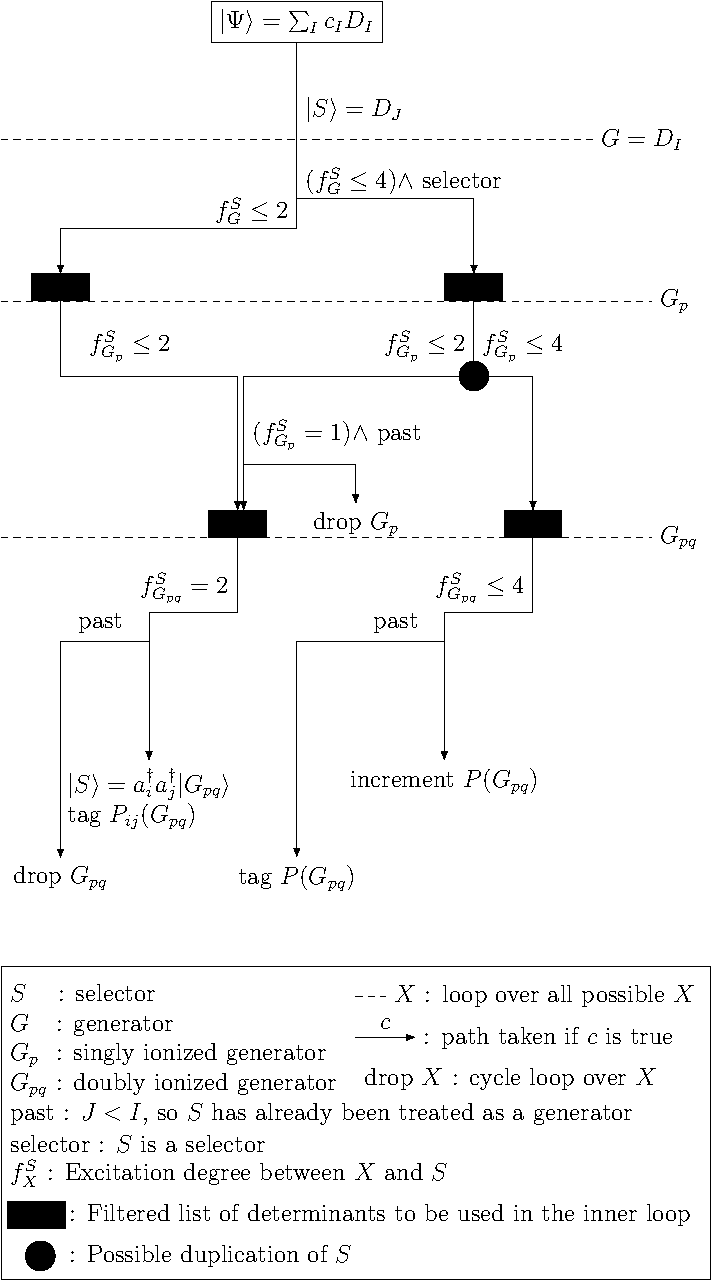
\includegraphics[height=0.90\textheight]{figures/cipsi/selection}
	\end{center}
        \caption{\label{fig:selection}
        $S$ is the selector currently flowing down the chart.
        Note that $M^{G_{pq}}$ is fully computed, and ``drop $G_{pq}$'' eventually reached, before any update is done to $P^{G_{pq}}$.
	}	
\end{figure}

Parallelisation \\
as seen, practical necessity to compute all alphas of the same generator at once \\
1 task = 1 generator, as simple \\

\end{document}
